\chapter{Introduction}\label{chap:introduction}
This paper is written for the master course \textit{Concepts of Programming Languages} of the apartment of computer science in the Winter Term 23/24 at the Technical University of Applied Sciences Rosenheim.
    \section{Background}\label{sec:background}
As of the TIOBE Index data as of November 2023, it is reported that there are currently over 150 programming languages in existence. This implies that, up until the present moment, the programming landscape continues to encompass a diverse array of languages, reflecting the dynamic and ever-evolving nature of the field.\cite{tiobeindex} The task of a programmer at a certain point in the production of software is to select one of these programming languages that is suitable for a particular problem. This can be a science in itself. This very topic has been discussed for around 50 years.\cite{Tharp1982}
The reason for that is that every language has its own paradigms and concepts. One can come up with a solution, selecting a language which fits a lot of problems but not a single one perfect. Or he selects one which fits perfect for a single problem but it is not possible to solve all the other problems.
So the goal would be to select the \textit{right} programming language which suits the requirements and the surrounding of the problem accordingly.
This spot should be covered by this paper with the comparison of Go and Haskell in the context of functional programming.

    \section{Purpose of the Project}\label{sec:purpose}
    The primary objective of this project is to analyse and explore the distinction and similarities between two languages within the realm of functional programming. The selected languages for this comparative study are Go\footnote{Website: \url{https://go.dev} (Accessed on 12/02/2023)} and Haskell\footnote{Website: \url{https://www.haskell.org} (Accessed on 12/02/2023)}. Go was chosen as the initial language due to its consistent usage throughout the course, making it mandatory inclusion in the project. 
    In addition to Go, a second programming language is essential for the comparative analysis, and Haskell has been selected for this purpose. The decision to include Haskell in this study is based on the author's deliberate choice, and the relationale behind this decision is elucidated in the subsequent section \ref{sec:whyhaskell}. By juxtaposing Go and Haskell, the project aims to unravel the nuances and divergences in their approaches to functional programming paradigms, shedding light on their distinctive features, strengths, and potential use cases. Through this comparative exploration, the project seeks to contribute valuable insights into the functional programming landscape, providing a nuanced understanding of the strengths and trade-offs associated with these two languages.

    \section{Why Haskell?}\label{sec:whyhaskell}
    One of the key reasons for choosing Haskell is its status as a pure functional programming language. In contrast to Go's multi-paradigm approach, Haskell's commitment to functional principles provides an excellent opportunity to explore the benefits of implementing code from a pure perspective.
    For a more in-depth understanding of Haskell, including its syntax, features, and functional programming principles, readers are encouraged to refer to section \ref{sec:haskell-overview}.

    \section{Roadmap}\label{sec:roadmap}
    Embedded within this exploration about functional programming is a brief discussion of the \textit{NerdDeck} Flash Card \ac{app} in chapter 2, our practical context for understanding functional programming in action. Besides of that this paper navigates a concise roadmap to compare functional programming in Go and Haskell, anchored by an initial overview of functional programming principles in chapter 3. It then swiftly transitions to individual language analyses in chapter 4, spotlighting key design philosophies and features of Go and Haskell. The centerpiece is chapter 5, a focused exploration of two critical functional concepts: Algebraic Data Types and Pattern Matching. Leveraging code examples, this section illuminates nuances in implementation, providing a succinct yet insightful comparative analysis. The paper concludes in chapter 6, summarizing challenges, key findings, and lessons learned from both the project and the comparative analysis. This streamlined roadmap ensures a comprehensive yet condensed examination of functional programming in Go and Haskell.

\chapter{Project Overview}\label{chap:project-overview}
    \section{Description of \textit{NerdDeck} Flash Card Application}\label{sec:description}
    The coding project which should illustrate and highlight similarities and differences about functional programming in Go and Haskell is a flash card \ac{app} called \textit{NerdDeck}. The \ac{app} should allow a single user to use the \ac{sm2} alorithm which is used for spaced recognition.\cite{sm2} Because \textit{NerdDeck} is build by a student, the requirements are also written from a students perspective. These should not differ too big from other users using this application.

    The program should act as a \ac{mvp}, so it's possible to do the comparison about functional programming. The goal is to implement this twice, one time in Go and then in Haskell, both in a functional style.

    \section{Requirements}
    \begin{table}[h]
        \centering
        \begin{tabular}{|m{0.5in}|m{4in}|}
            \hline
            \textbf{ID} & \textbf{Requirement} \\
            \hline
            1 & As a student, I want to create a flashcard with a question on the front and an answer on the back. \\
            \hline
            2 & As a student, I want to create a deck of flashcards. \\
            \hline
            3 & As a student, I want to assign a flashcard to a deck while creating it. \\
            \hline
            4 & As a student, I want to be able to create multiple decks. \\
            \hline
            5 & As a student, I want to view my flashcards. \\
            \hline
            6 & As a student, I want to delete my flashcards. \\
            \hline
            7 & As a student, I want to apply spaced repetition. \\
            \hline
        \end{tabular}
        \caption{\textit{NerdDeck} Requirements}
        \label{tab:requirements}
    \end{table}

    \section{Data}
    For the purpose of this project, a single \ac{json} file is used as a simple and lightweight database to store flashcards. While this approach is suitable for educational and illustrative purposes, it may not be suitable for production usage due to limitations in scalability and concurrent access. In a production environment, a more robust database solution should be considered, such as a relational database (e.g., PostgreSQL\footnote{Website: \url{https://www.postgresql.org} (Accessed on 12/02/2023)}, MySQL\footnote{Website: \url{https://www.mysql.com} (Accessed on 12/02/2023)}) or a NoSQL database (e.g., MongoDB\footnote{Website: \url{https://www.mongodb.com} (Accessed on 12/02/2023)}). The choice of the database will depend on the specific requirements of the \ac{app}.

    \subsection{Model}
    To be able to fulfill certain requirements a model is needed for both a flashcard and also for a deck. These are shown in figure \ref{fig:er-model}. It is important that a deck can contain multiple flashcards while a flashcard always remain to a single deck. This model should be used within both languages.

    \begin{figure}
        \centering
        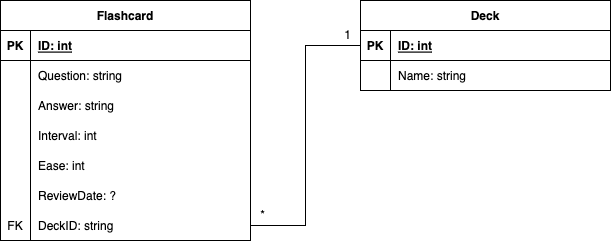
\includegraphics[width=1\textwidth]{NerddeckModel.png}
        \caption{Entity-Relationship Model of Flashcard and Deck}
        \label{fig:er-model}
    \end{figure}

    \begin{lstlisting}[language=json,firstnumber=1,float=tp, caption={Example of how a flashcard is saved inside a \ac{json} file}, label=l:flashcardjson]
    [
    {
        "Question": "What is functional programming?",
        "Answer": "Functional programming is a programming paradigm that treats computation as the evaluation of mathematical functions and avoids changing-state and mutable data.",
        "Interval": 1,
        "Ease": 1,
        "ReviewDate: ?,
        "DeckID: ""
    }
    ]
        
    \end{lstlisting}


\chapter{Overview of functional programming}\label{chap:functional-programming}
Functional programming was first introduced in 1950 in the impure programming language LISP. There are existing pure functional languages like Haskell and impure functional languages like Go.

Imperitive vs delative programming.

In the past as well as today, the motivation for developing software with the functional paradigm is while software becomes more and more complex, the importance for a good structure is getting more important.\cite{Hughes1989}

It is necessary to mention that there are lots of principles associated with functional programming. In the following an overview will be given over the most important ones: Purity, Higher-order functions, Lazy Evaluation, Pattern Matching, Algebraic Datatypes.

\begin{shaded}
    \noindent
    \glqq{}Functional programming is so called because a program consists entirely of functions.\grqq{} \cite{Hughes1989}
\end{shaded}
Another formulation for this is that functions are treated as first-class citizens.

    \section{Key principles}
        \subsection{Purity}
        There are no side effects.

        \subsection{Higher-order functions}
        Use functions as parameters and return values.

        \subsection{Lazy evaluation}
        Only evaluate a value if necessary.

        \subsection{Algebraic data types}
        For example sum- and producttypes. These will be discussed more in detail in section \ref{sec:algebraic-data-types}

        \subsection{Pattern Matching}
        This will be more discussed in detail in section \ref{sec:pattern-matching}


\chapter{Introduction to Go and Haskell}\label{chap:language-comparison}
In this chapter, we delve into the distinctive features of Go and Haskell, offering a brief overview of each language before embarking on comparative analysis.

    \section{Overview of Go}\label{sec:go-overview}
    The usage of the programming language Go allows to build simple, secure and scalable systems. It is used very widely within big companys like Google, Paypal or Netflix. Besides of that it is open source. \cite{GoWebsite}
    \section{Overview of Haskell}\label{sec:haskell-overview}
    Haskell is used for the comparison to Go because it is a pure functional programming language.
    For the overview of Haskell the book \textit{Effective Haskell: Solving Real-World Problems with Strongly Typed Functional Programming} \cite{Skinner} will be used.
    The first Haskell language report was published in 1990 by Paul Hudak and Philip Wadler. It is named after the mathematician Haskell Brooks Curry.\cite{Hudak2007}

    \section{Comparative Analysis}\label{sec:comparative-analysis}


\chapter{Comparison of functional concepts}
    \section{Algebraic Data Types}\label{sec:algebraic-data-types}
    \section{Pattern Matching}\label{sec:pattern-matching}

\chapter{Conclusion}\label{chap:conclusion}
    \section{Challenges}\label{sec:challenges}
    \section{Summary of Findings}\label{sec:findings-summary}
    \section{Lessons Learned}\label{sec:lessons-learned}
